\documentclass[twoside]{book}

% Packages required by doxygen
\usepackage{fixltx2e}
\usepackage{calc}
\usepackage{doxygen}
\usepackage[export]{adjustbox} % also loads graphicx
\usepackage{graphicx}
\usepackage[utf8]{inputenc}
\usepackage{makeidx}
\usepackage{multicol}
\usepackage{multirow}
\PassOptionsToPackage{warn}{textcomp}
\usepackage{textcomp}
\usepackage[nointegrals]{wasysym}
\usepackage[table]{xcolor}

% Font selection
\usepackage[T1]{fontenc}
\usepackage[scaled=.90]{helvet}
\usepackage{courier}
\usepackage{amssymb}
\usepackage{sectsty}
\renewcommand{\familydefault}{\sfdefault}
\allsectionsfont{%
  \fontseries{bc}\selectfont%
  \color{darkgray}%
}
\renewcommand{\DoxyLabelFont}{%
  \fontseries{bc}\selectfont%
  \color{darkgray}%
}
\newcommand{\+}{\discretionary{\mbox{\scriptsize$\hookleftarrow$}}{}{}}

% Page & text layout
\usepackage{geometry}
\geometry{%
  a4paper,%
  top=2.5cm,%
  bottom=2.5cm,%
  left=2.5cm,%
  right=2.5cm%
}
\tolerance=750
\hfuzz=15pt
\hbadness=750
\setlength{\emergencystretch}{15pt}
\setlength{\parindent}{0cm}
\setlength{\parskip}{3ex plus 2ex minus 2ex}
\makeatletter
\renewcommand{\paragraph}{%
  \@startsection{paragraph}{4}{0ex}{-1.0ex}{1.0ex}{%
    \normalfont\normalsize\bfseries\SS@parafont%
  }%
}
\renewcommand{\subparagraph}{%
  \@startsection{subparagraph}{5}{0ex}{-1.0ex}{1.0ex}{%
    \normalfont\normalsize\bfseries\SS@subparafont%
  }%
}
\makeatother

% Headers & footers
\usepackage{fancyhdr}
\pagestyle{fancyplain}
\fancyhead[LE]{\fancyplain{}{\bfseries\thepage}}
\fancyhead[CE]{\fancyplain{}{}}
\fancyhead[RE]{\fancyplain{}{\bfseries\leftmark}}
\fancyhead[LO]{\fancyplain{}{\bfseries\rightmark}}
\fancyhead[CO]{\fancyplain{}{}}
\fancyhead[RO]{\fancyplain{}{\bfseries\thepage}}
\fancyfoot[LE]{\fancyplain{}{}}
\fancyfoot[CE]{\fancyplain{}{}}
\fancyfoot[RE]{\fancyplain{}{\bfseries\scriptsize Generated by Doxygen }}
\fancyfoot[LO]{\fancyplain{}{\bfseries\scriptsize Generated by Doxygen }}
\fancyfoot[CO]{\fancyplain{}{}}
\fancyfoot[RO]{\fancyplain{}{}}
\renewcommand{\footrulewidth}{0.4pt}
\renewcommand{\chaptermark}[1]{%
  \markboth{#1}{}%
}
\renewcommand{\sectionmark}[1]{%
  \markright{\thesection\ #1}%
}

% Indices & bibliography
\usepackage{natbib}
\usepackage[titles]{tocloft}
\setcounter{tocdepth}{3}
\setcounter{secnumdepth}{5}
\makeindex

% Hyperlinks (required, but should be loaded last)
\usepackage{ifpdf}
\ifpdf
  \usepackage[pdftex,pagebackref=true]{hyperref}
\else
  \usepackage[ps2pdf,pagebackref=true]{hyperref}
\fi
\hypersetup{%
  colorlinks=true,%
  linkcolor=blue,%
  citecolor=blue,%
  unicode%
}

% Custom commands
\newcommand{\clearemptydoublepage}{%
  \newpage{\pagestyle{empty}\cleardoublepage}%
}

\usepackage{caption}
\captionsetup{labelsep=space,justification=centering,font={bf},singlelinecheck=off,skip=4pt,position=top}

%===== C O N T E N T S =====

\begin{document}

% Titlepage & ToC
\hypersetup{pageanchor=false,
             bookmarksnumbered=true,
             pdfencoding=unicode
            }
\pagenumbering{roman}
\begin{titlepage}
\vspace*{7cm}
\begin{center}%
{\Large Eta\+Gen }\\
\vspace*{1cm}
{\large Generated by Doxygen 1.8.11}\\
\end{center}
\end{titlepage}
\clearemptydoublepage
\tableofcontents
\clearemptydoublepage
\pagenumbering{arabic}
\hypersetup{pageanchor=true}

%--- Begin generated contents ---
\chapter{Eta\+Gen}
\label{index}\hypertarget{index}{}An event trigger generator based on Hilbert-\/\+Huang Transform~\newline
 It is a Python module but the core library of Eta\+Gen is built in C/\+C++

\subsection*{Dependences}


\begin{DoxyItemize}
\item Numpy $>$= 1.\+10
\item Boost.\+Python $<$ 1.\+65 or $>$= 1.\+64 with Boost.\+Numpy
\end{DoxyItemize}

\#\# Install 
\begin{DoxyCode}
1 $ python setup.py install --user
\end{DoxyCode}


\subsection*{Sample U\+S\+A\+GE\+:}


\begin{DoxyItemize}
\item This shows how to generate event triggers from {\itshape data} by Eta\+Gen~\newline
 
\begin{DoxyCode}
1 >>> from etagen import etagen, kernel
2 
3 >>> h = etagen(data, fsr=1024)
4 
5 >>> h.set\_emd\_param(num\_imfs=8, num\_sifts=15, S\_number=1, emd\_size=1024, num\_seg=4,
       w\_type=kernel.SIN\_KERNEL)
6 
7 >>> h.show\_emd\_param()<br>
8 Parameters are set as follows.<br>
9 [General]<br>
10 Number of IMFs: 8<br>
11 Number of siftings:     15<br>
12 S-Number:       1<br>
13 [wSEMD settings]<br>
14 EMD size:       1024<br>
15 Number of segments:     4
16 
17 >>> h.wsemd()
18 
19 >>> h.hilbert(filter\_length=128, stride=1024)
20 
21 >>> h.get\_utriggers(snr\_th=5, stride=4*fsr, overlap=2*fsr)<br>
22 Generating triggers with 5-snr threshold in segments of length 4096, overlapping 2048 samples and skipping
       0 samples from boundaries...<br>
23 ... generated 25 trigger event(s)
24 
25 >>> h.get\_triggers(t\_tolerance=0.001, f\_tolerance=0.5, snr\_th=5.5)<br>
26 u\_snr\_th should be larger than the one used to generate triggers: assuming u\_snr\_th = 5<br>
27 Clustering triggers of u\_snr > 5 with time tolerance=0.001, frequency tolerance=0.5 and dropping clusters
       of snr < 5.5...<br>
28 total Clusters : 25 > 5.500000<br>
29 total Clusters : 12 > 5.500000<br>
30 ... generated 12 trigger cluster(s)
31 
32 >>> h.trgs[['c\_time','c\_freq','p\_time','p\_freq','npts','snr']]<br>
33 array([ (0.041015625, 297.67912076702106, 0.041015625, 297.67912076702106, 1, 5.546819634000152),<br>
34    (0.6464843749999999, 344.6262005898434, 0.646484375, 344.6262005898434, 1, 5.797973757254617),<br>
35    (1.2744140625, 260.1084208607948, 1.2744140625, 260.1084208607948, 1, 5.546288486345601),<br>
36    (1.5664062499999998, 142.61211763115602, 1.56640625, 142.61211763115602, 1, 6.513913449375204),<br>
37    (1.8193359374999998, 333.3958253278954, 1.8193359375, 333.39582532789547, 1, 6.632835601773412),<br>
38    (2.7138671875, 341.5032411355364, 2.7138671875, 341.5032411355364, 1, 6.609969624271628),<br>
39    (4.1552734375, 220.52834605967874, 4.1552734375, 220.5283460596787, 1, 5.8852032771220015),<br>
40    (4.493164062499999, 201.227897198888, 4.4931640625, 201.22789719888803, 1, 5.890950833813454),<br>
41    (5.766601562500001, 229.12911997930595, 5.7666015625, 229.12911997930595, 1, 5.557695477749056),<br>
42    (6.659179687499999, 245.8274380780258, 6.6591796875, 245.8274380780258, 1, 5.8990177018284875),<br>
43    (6.328125, 34.86349503817338, 6.328125, 34.86349503817338, 1, 5.834112766561207),<br>
44    (6.0, 67.39566743927662, 6.0, 67.39566743927662, 1, 5.9916237288573955)], <br>
45   dtype=[('c\_time', '<f8'), ('c\_freq', '<f8'), ('p\_time', '<f8'), ('p\_freq', '<f8'), ('npts', '<i8'),
       ('snr', '<f8')])
\end{DoxyCode}
 
\end{DoxyItemize}
\chapter{Hierarchical Index}
\section{Class Hierarchy}
This inheritance list is sorted roughly, but not completely, alphabetically\+:\begin{DoxyCompactList}
\item etagen\begin{DoxyCompactList}
\item \contentsline{section}{python.\+\_\+wrap.\+etagen}{\pageref{classpython_1_1__wrap_1_1etagen}}{}
\end{DoxyCompactList}
\end{DoxyCompactList}

\chapter{Class Index}
\section{Class List}
Here are the classes, structs, unions and interfaces with brief descriptions\+:\begin{DoxyCompactList}
\item\contentsline{section}{\hyperlink{classpython_1_1__wrap_1_1etagen}{python.\+\_\+wrap.\+etagen} }{\pageref{classpython_1_1__wrap_1_1etagen}}{}
\end{DoxyCompactList}

\chapter{Class Documentation}
\hypertarget{classpython_1_1__wrap_1_1etagen}{\section{python.\-\_\-wrap.\-etagen Class Reference}
\label{classpython_1_1__wrap_1_1etagen}\index{python.\-\_\-wrap.\-etagen@{python.\-\_\-wrap.\-etagen}}
}
Inheritance diagram for python.\-\_\-wrap.\-etagen\-:\begin{figure}[H]
\begin{center}
\leavevmode
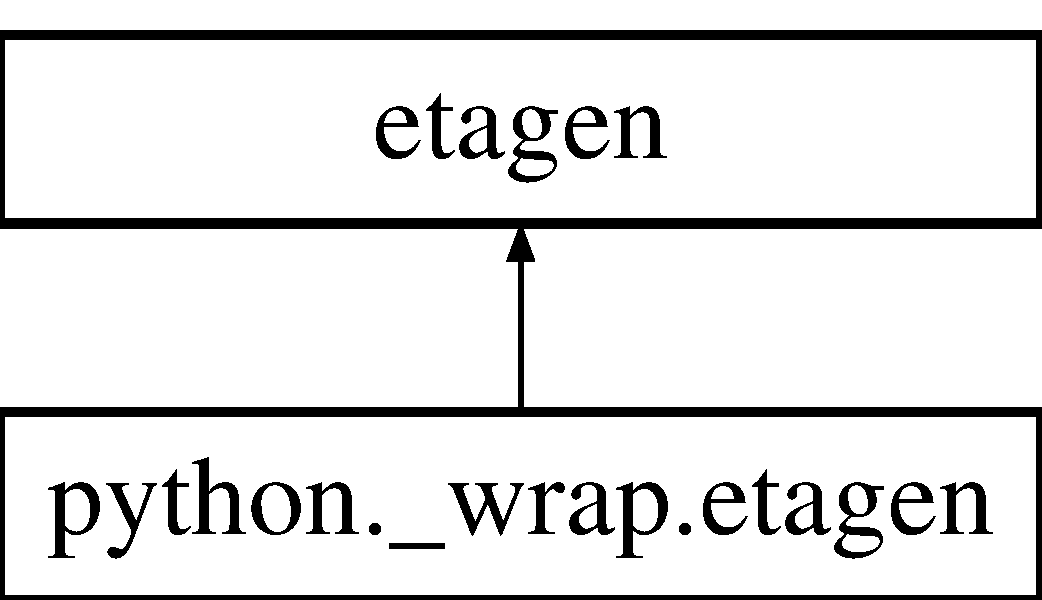
\includegraphics[height=2.000000cm]{classpython_1_1__wrap_1_1etagen}
\end{center}
\end{figure}
\subsection*{Public Member Functions}
\begin{DoxyCompactItemize}
\item 
def \hyperlink{classpython_1_1__wrap_1_1etagen_a27945aeb4059ba3b81e38fff12ea5424}{get\-\_\-utriggers}
\item 
def \hyperlink{classpython_1_1__wrap_1_1etagen_a73614979353f43ac4bfc923bce68d2cd}{get\-\_\-utriggers\-\_\-from\-\_\-file}
\item 
def \hyperlink{classpython_1_1__wrap_1_1etagen_a6f332e2242c9bb8b87dc593f17542873}{get\-\_\-triggers}
\item 
def \hyperlink{classpython_1_1__wrap_1_1etagen_add5689086be59da228ee79535f19aa8a}{get\-\_\-triggers\-\_\-from\-\_\-file}
\item 
def \hyperlink{classpython_1_1__wrap_1_1etagen_adba206932fb4791a553a36d147c43bd8}{copy}
\item 
def \hyperlink{classpython_1_1__wrap_1_1etagen_a5393c44d9e6a8754dda3a3835f66cebb}{plot\-\_\-tfd}
\item 
def \hyperlink{classpython_1_1__wrap_1_1etagen_aa8188f4111faefd7df20a40e7a233afd}{plot\-\_\-trgs}
\end{DoxyCompactItemize}
\subsection*{Public Attributes}
\begin{DoxyCompactItemize}
\item 
\hypertarget{classpython_1_1__wrap_1_1etagen_ade022a3ddd38334c6a1c4666e4b791e2}{{\bfseries min\-\_\-snr}}\label{classpython_1_1__wrap_1_1etagen_ade022a3ddd38334c6a1c4666e4b791e2}

\item 
\hypertarget{classpython_1_1__wrap_1_1etagen_a64f39feb7baa26e4a048455eea79672f}{{\bfseries std}}\label{classpython_1_1__wrap_1_1etagen_a64f39feb7baa26e4a048455eea79672f}

\item 
\hypertarget{classpython_1_1__wrap_1_1etagen_a8d72e02eb9ef5898d29e07a4f8bf35f7}{{\bfseries trg\-\_\-skip}}\label{classpython_1_1__wrap_1_1etagen_a8d72e02eb9ef5898d29e07a4f8bf35f7}

\item 
\hypertarget{classpython_1_1__wrap_1_1etagen_aedc63ca3e4633696c1d1432ae5af65e7}{{\bfseries trg\-\_\-stride}}\label{classpython_1_1__wrap_1_1etagen_aedc63ca3e4633696c1d1432ae5af65e7}

\item 
\hypertarget{classpython_1_1__wrap_1_1etagen_abef066c8bcca998720ed758824cc27c0}{{\bfseries trg\-\_\-overlap}}\label{classpython_1_1__wrap_1_1etagen_abef066c8bcca998720ed758824cc27c0}

\item 
\hypertarget{classpython_1_1__wrap_1_1etagen_ab9a3023653e8bc4fa767509c1f0cbb18}{{\bfseries utrgs}}\label{classpython_1_1__wrap_1_1etagen_ab9a3023653e8bc4fa767509c1f0cbb18}

\item 
\hypertarget{classpython_1_1__wrap_1_1etagen_afdf0a29439d61d5226ba044da470edf0}{{\bfseries u\-\_\-snr\-\_\-threshold}}\label{classpython_1_1__wrap_1_1etagen_afdf0a29439d61d5226ba044da470edf0}

\item 
\hypertarget{classpython_1_1__wrap_1_1etagen_a7f8badecd73f47578c62974a0e74080d}{{\bfseries snr\-\_\-threshold}}\label{classpython_1_1__wrap_1_1etagen_a7f8badecd73f47578c62974a0e74080d}

\item 
\hypertarget{classpython_1_1__wrap_1_1etagen_a3f69ad9121ced6715a6a3e52de40536e}{{\bfseries trgs}}\label{classpython_1_1__wrap_1_1etagen_a3f69ad9121ced6715a6a3e52de40536e}

\end{DoxyCompactItemize}
\subsection*{Static Public Attributes}
\begin{DoxyCompactItemize}
\item 
\hypertarget{classpython_1_1__wrap_1_1etagen_abd7912f308ef9623da9dfcea0e8a1c95}{list {\bfseries utrg\-\_\-dtype} = \mbox{[}('imf\-\_\-idx',int), ('s\-\_\-time',float), ('e\-\_\-time',float), ('p\-\_\-time',float), ('p\-\_\-amp',float), ('p\-\_\-freq',float), ('f\-\_\-min',float), ('f\-\_\-max',float), ('snr',float)\mbox{]}}\label{classpython_1_1__wrap_1_1etagen_abd7912f308ef9623da9dfcea0e8a1c95}

\item 
\hypertarget{classpython_1_1__wrap_1_1etagen_a9e04218bd2d74e12cc0a91f5f8fd0bc1}{list {\bfseries trg\-\_\-dtype} = \mbox{[}('s\-\_\-time',float), ('e\-\_\-time',float), ('c\-\_\-time',float), ('c\-\_\-freq',float), ('c\-\_\-energy',float), ('p\-\_\-time',float), ('p\-\_\-freq',float), ('p\-\_\-amp',float), ('p\-\_\-imf\-\_\-idx',int), ('p\-\_\-snr',float), ('f\-\_\-min',float), ('f\-\_\-max',float), ('npts',int), ('snr\-\_\-rss',float), ('snr',float)\mbox{]}}\label{classpython_1_1__wrap_1_1etagen_a9e04218bd2d74e12cc0a91f5f8fd0bc1}

\end{DoxyCompactItemize}


\subsection{Member Function Documentation}
\hypertarget{classpython_1_1__wrap_1_1etagen_adba206932fb4791a553a36d147c43bd8}{\index{python\-::\-\_\-wrap\-::etagen@{python\-::\-\_\-wrap\-::etagen}!copy@{copy}}
\index{copy@{copy}!python::_wrap::etagen@{python\-::\-\_\-wrap\-::etagen}}
\subsubsection[{copy}]{\setlength{\rightskip}{0pt plus 5cm}def python.\-\_\-wrap.\-etagen.\-copy (
\begin{DoxyParamCaption}
\item[{}]{self, }
\item[{}]{start = {\ttfamily None}, }
\item[{}]{end = {\ttfamily None}}
\end{DoxyParamCaption}
)}}\label{classpython_1_1__wrap_1_1etagen_adba206932fb4791a553a36d147c43bd8}
\begin{DoxyVerb}hhtout = self.copy(start=None, end=None):

Copy HHT instance [from *start* second to *end* second, if specified]
*start*/*end* should be greater than self.start_time

Input parameters:

    start       start time to copy the data
    end     end time to copy the data

Output parameters:

    hhtout      copied HHT instance
\end{DoxyVerb}
 \hypertarget{classpython_1_1__wrap_1_1etagen_a6f332e2242c9bb8b87dc593f17542873}{\index{python\-::\-\_\-wrap\-::etagen@{python\-::\-\_\-wrap\-::etagen}!get\-\_\-triggers@{get\-\_\-triggers}}
\index{get\-\_\-triggers@{get\-\_\-triggers}!python::_wrap::etagen@{python\-::\-\_\-wrap\-::etagen}}
\subsubsection[{get\-\_\-triggers}]{\setlength{\rightskip}{0pt plus 5cm}def python.\-\_\-wrap.\-etagen.\-get\-\_\-triggers (
\begin{DoxyParamCaption}
\item[{}]{self, }
\item[{}]{snr\-\_\-th = {\ttfamily 10}, }
\item[{}]{t\-\_\-tolerance = {\ttfamily 0.}, }
\item[{}]{f\-\_\-tolerance = {\ttfamily 0.}, }
\item[{}]{u\-\_\-snr\-\_\-th = {\ttfamily 3}}
\end{DoxyParamCaption}
)}}\label{classpython_1_1__wrap_1_1etagen_a6f332e2242c9bb8b87dc593f17542873}
\begin{DoxyVerb}self.get_triggers(maxDist=2):

Cluster trigger events generated by self.get_utriggers().

Required item:

    self.utrgs  triggers generated by self.get_utriggers()

Input parameters:

    maxDist     maximum distance to cluster tiggers. Default is 2.
    unit_time   unit time for distance. Default is 0.01(=10ms).
    u_snr_th    A threshold parameter for each trigger event. Default is 3.
    snr_th  A threshold parameter for a cluster of triggers.
    Default is 10.
    
Output:

    self.utrgs  The trigger information generated if not calculated before.
    The information is [IMF index, start time, end time,
    peak time, peak amplitude, peak frequency, snr].
    self.trgs   The trigger cluster information generated.
\end{DoxyVerb}
 \hypertarget{classpython_1_1__wrap_1_1etagen_add5689086be59da228ee79535f19aa8a}{\index{python\-::\-\_\-wrap\-::etagen@{python\-::\-\_\-wrap\-::etagen}!get\-\_\-triggers\-\_\-from\-\_\-file@{get\-\_\-triggers\-\_\-from\-\_\-file}}
\index{get\-\_\-triggers\-\_\-from\-\_\-file@{get\-\_\-triggers\-\_\-from\-\_\-file}!python::_wrap::etagen@{python\-::\-\_\-wrap\-::etagen}}
\subsubsection[{get\-\_\-triggers\-\_\-from\-\_\-file}]{\setlength{\rightskip}{0pt plus 5cm}def python.\-\_\-wrap.\-etagen.\-get\-\_\-triggers\-\_\-from\-\_\-file (
\begin{DoxyParamCaption}
\item[{}]{self, }
\item[{}]{trg\-\_\-file, }
\item[{}]{kwargs}
\end{DoxyParamCaption}
)}}\label{classpython_1_1__wrap_1_1etagen_add5689086be59da228ee79535f19aa8a}
\begin{DoxyVerb}self.get_triggers_from_file(trg_file, **kwargs):

Read clustered trigger events from file

Input parameters:

    trg_file    Filename that contains clustered trigger informations
    in ASCII format
    **kwargs    kwargs for numpy.loadtxt or numpy.fromfile
    
Output:

    self.trgs   The trigger cluster information generated.
\end{DoxyVerb}
 \hypertarget{classpython_1_1__wrap_1_1etagen_a27945aeb4059ba3b81e38fff12ea5424}{\index{python\-::\-\_\-wrap\-::etagen@{python\-::\-\_\-wrap\-::etagen}!get\-\_\-utriggers@{get\-\_\-utriggers}}
\index{get\-\_\-utriggers@{get\-\_\-utriggers}!python::_wrap::etagen@{python\-::\-\_\-wrap\-::etagen}}
\subsubsection[{get\-\_\-utriggers}]{\setlength{\rightskip}{0pt plus 5cm}def python.\-\_\-wrap.\-etagen.\-get\-\_\-utriggers (
\begin{DoxyParamCaption}
\item[{}]{self, }
\item[{}]{snr\-\_\-th = {\ttfamily 3}, }
\item[{}]{stride = {\ttfamily 0}, }
\item[{}]{overlap = {\ttfamily 0}, }
\item[{}]{skip = {\ttfamily 0}}
\end{DoxyParamCaption}
)}}\label{classpython_1_1__wrap_1_1etagen_a27945aeb4059ba3b81e38fff12ea5424}
\begin{DoxyVerb}self.get_utriggers(snr_th=3, stride=0, overlap=0, skip=0):

Generate triggers, provided that Intrinsic Mode Functions(IMFs) are
obtained before self.get_utriggers() is called.

Required item:

    self.imfs   IMFs obtained by self.get_imfs()

Input parameters:

    s       A threshold parameter. Default is 3.
    stride      The length of segment in which triggers are generated.
    overlap     The length of overlap of two neighboring segments.
    skip        The length of skipped samples at boundaries of IMFs.
    
Output:

    self.utrgs  The trigger information generated.
    The information is [IMF index, start time, end time,
    peak time, peak amplitude, peak frequency, snr].
\end{DoxyVerb}
 \hypertarget{classpython_1_1__wrap_1_1etagen_a73614979353f43ac4bfc923bce68d2cd}{\index{python\-::\-\_\-wrap\-::etagen@{python\-::\-\_\-wrap\-::etagen}!get\-\_\-utriggers\-\_\-from\-\_\-file@{get\-\_\-utriggers\-\_\-from\-\_\-file}}
\index{get\-\_\-utriggers\-\_\-from\-\_\-file@{get\-\_\-utriggers\-\_\-from\-\_\-file}!python::_wrap::etagen@{python\-::\-\_\-wrap\-::etagen}}
\subsubsection[{get\-\_\-utriggers\-\_\-from\-\_\-file}]{\setlength{\rightskip}{0pt plus 5cm}def python.\-\_\-wrap.\-etagen.\-get\-\_\-utriggers\-\_\-from\-\_\-file (
\begin{DoxyParamCaption}
\item[{}]{self, }
\item[{}]{trg\-\_\-file, }
\item[{}]{kwargs}
\end{DoxyParamCaption}
)}}\label{classpython_1_1__wrap_1_1etagen_a73614979353f43ac4bfc923bce68d2cd}
\begin{DoxyVerb}self.get_utriggers_from_file(trg_file, **kwargs):

Read triggers from file

Input parameters:

    trg_file    Filename that contains trigger informations in ASCII format
    **kwargs    kwargs for numpy.loadtxt or numpy.fromfile
    
Output:

    self.utrgs  The trigger information generated.
    The information is [IMF index, start time, end time,
    peak time, peak amplitude, peak frequency, snr].
\end{DoxyVerb}
 \hypertarget{classpython_1_1__wrap_1_1etagen_a5393c44d9e6a8754dda3a3835f66cebb}{\index{python\-::\-\_\-wrap\-::etagen@{python\-::\-\_\-wrap\-::etagen}!plot\-\_\-tfd@{plot\-\_\-tfd}}
\index{plot\-\_\-tfd@{plot\-\_\-tfd}!python::_wrap::etagen@{python\-::\-\_\-wrap\-::etagen}}
\subsubsection[{plot\-\_\-tfd}]{\setlength{\rightskip}{0pt plus 5cm}def python.\-\_\-wrap.\-etagen.\-plot\-\_\-tfd (
\begin{DoxyParamCaption}
\item[{}]{self, }
\item[{}]{indices = {\ttfamily None}, }
\item[{}]{kwargs}
\end{DoxyParamCaption}
)}}\label{classpython_1_1__wrap_1_1etagen_a5393c44d9e6a8754dda3a3835f66cebb}
\begin{DoxyVerb}self.plot_tfd(indices=None, **kwargs):

Plot time-frequency-distribution (TFD)

Input parameters:

    indices     List of indices of IMFs used for plotting TFD
    All IMFs will be used by default.
    **kwargs    kwargs for matplotlib.pyplot.scatter
\end{DoxyVerb}
 \hypertarget{classpython_1_1__wrap_1_1etagen_aa8188f4111faefd7df20a40e7a233afd}{\index{python\-::\-\_\-wrap\-::etagen@{python\-::\-\_\-wrap\-::etagen}!plot\-\_\-trgs@{plot\-\_\-trgs}}
\index{plot\-\_\-trgs@{plot\-\_\-trgs}!python::_wrap::etagen@{python\-::\-\_\-wrap\-::etagen}}
\subsubsection[{plot\-\_\-trgs}]{\setlength{\rightskip}{0pt plus 5cm}def python.\-\_\-wrap.\-etagen.\-plot\-\_\-trgs (
\begin{DoxyParamCaption}
\item[{}]{self, }
\item[{}]{indices = {\ttfamily None}, }
\item[{}]{clustered = {\ttfamily True}, }
\item[{}]{scale = {\ttfamily True}, }
\item[{}]{kwargs}
\end{DoxyParamCaption}
)}}\label{classpython_1_1__wrap_1_1etagen_aa8188f4111faefd7df20a40e7a233afd}
\begin{DoxyVerb}self.plot_trgs(indices=None, **kwargs):

Plot trigger-gram

Input parameters:

    indices     List of indices of triggers used for plotting trigger-gram
    All triggers will be used by default.
    **kwargs    kwargs for matplotlib.pyplot.scatter
\end{DoxyVerb}
 

The documentation for this class was generated from the following file\-:\begin{DoxyCompactItemize}
\item 
\-\_\-wrap.\-py\end{DoxyCompactItemize}

%--- End generated contents ---

% Index
\backmatter
\newpage
\phantomsection
\clearemptydoublepage
\addcontentsline{toc}{chapter}{Index}
\printindex

\end{document}
